The following subchapters develop the theoretical foundations necessary for understanding and
designing a demonstrator for the \acrshort{tof} method.

\subsection{Time of Flight}

The measurement method known as \dq \acrlong{tof}\dq\ involves measuring the transit time of a signal.
The signal can be either optical or acoustic. One application of this is, for example, distance measurement.

In the optical principle discussed here, a transmitter emits light that is detected by a receiver.
A time measurement can be made between the sending and receiving of the signal. Because light propagates at a defined
speed, this time measurement can be used to determine the distance
the signal has traveled within the measured time.

\begin{figure}[H]
    \centering
    \includegraphics[width=\textwidth]{../diagrams/dToF_vs_iToF.pdf}
    \caption{Visualization of a: direct \acrshort{tof} and b: indirect \acrshort{tof}}\label{fig:dtof_vs_itof}
\end{figure}

There are two types of \acrshort{tof}: direct \acrshort{tof} (dToF) and indirect \acrshort{tof} (iToF). With dToF
only the time between the transmission and reception pulse is determined. In the figure~\ref{fig:dtof_vs_itof},
such pulses are shown at a).

In iToF, the phase shift of a modulated light signal is also measured (in some cases additionally) to the runtime measurement.
This is shown in figure~\ref{fig:dtof_vs_itof} in part b). This method allows higher resolutions to
be achieved, but is much more complex in terms of evaluation and signal processing.

This work is limited to the direct \acrshort{tof} method.

In the following, the theoretical principles, especially with regard to designing a suitable optical system, are discussed.

\pagebreak

\subsection{Photocurrent}

To calculate the theoretically expected photocurrent, a distance of $10~m$ from the wall is assumed.

In a simplified consideration, a laser beam with a divergence of $0\degree$ hits a wall at right angles
and is scattered uniformly in a hemisphere. In reality, the laser will not hit the wall at $0\degree$ and
the scattering will not be uniform, but rather more concentrated in the center.

The calculation of the received radiant power, the radiant intensity, the solid angle of a hemisphere, and the
photocurrent are shown in formulas~\ref{eq:pin}, \ref{eq:ie}, \ref{eq:omega} and \ref{eq:iph}, respectively.

\begin{equation}\label{eq:pin}
    P_{in} = E_e \cdot A = \frac{I_e}{r^2} \cdot A
\end{equation}
\myequations{Incoming light power}

\begin{equation}\label{eq:ie}
    I_e = \frac{P_{out}}{\Omega}
\end{equation}
\myequations{Radiation intensity}

\begin{equation}\label{eq:omega}
    \Omega = 4\cdot \pi \cdot 0.5
\end{equation}
\myequations{solid angle}

\begin{equation}\label{eq:iph}
    I_{ph} = S \cdot P_{in}
\end{equation}
\myequations{photocurrent}

\subsubsection{Calculation with RLD94PZJ5 and BPV23NF}

Initial calculations are carried out with the RLD94PZJ5 laser diode \cite{rohm2020rld94pzj5_datasheet} and the BPV23NF photodiode
\cite{vishay2024bpv23nf_datasheet}.

The relevant values from the data sheets are listed in formula~\ref{eq:rld94pzj5_num} and \ref{eq:rbpv23nf_num}.

\begin{equation}\label{eq:rld94pzj5_num}
    P_{out} = 285~mW
\end{equation}
\myequations{Values of the RLD94PZJ5}

\begin{equation}\label{eq:rbpv23nf_num}
    \begin{split}
        A & = 4.4~mm^2        \\
        S & = 0.6~\frac{A}{W}
    \end{split}
\end{equation}
\myequations{Values of BPV23NF}

These values inserted in formula~\ref{eq:ie}, \ref{eq:pin} and \ref{eq:iph} yield the results in
formula~\ref{eq:rld94pzj5_rbpv23nf_num}.

\begin{equation}\label{eq:rld94pzj5_rbpv23nf_num}
    \begin{split}
        I_e    & = \frac{P_{out}}{\Omega} = \frac{285~mW}{4\cdot \pi \cdot 0.5~sr} = 45.4~\frac{mW}{sr} \\
        P_{in} & = \frac{I_e}{r^2} \cdot A = \frac{45.4~\frac{mW}{sr}}{(10~m)^2} \cdot 4.4~mm^2 = 2~nW  \\
        I_{ph} & = S \cdot P_{in} = 0.6~\frac{A}{W} \cdot 2~nW = 1.2~nA
    \end{split}
\end{equation}
\myequations{Numerical results with RLD94PZJ5 and BPV23NF}

\subsubsection{Calculation with RLD65NZX1 and NJL6401R-3}

The laser diode RLD94PZJ5 has two disadvantages with regard to this project work: on the one hand, it has such a high power that
it can be harmful to the human eye. On the other hand, it emits in a wavelength range that
is not visible to the human eye.

For these reasons, a second laser diode is being evaluated: RLD65NZX1 \cite{rohm2019rld65nzx1_datasheet}. It is paired
with the photodiode NJL6401R-3 \cite{jrc2014njl6401r3_datasheet}. The following calculations are based on
these two components.

The relevant values from the data sheets are listed in formula~\ref{eq:rld65nzx1_num} and \ref{eq:njl6401r3_num}.

\begin{equation}\label{eq:rld65nzx1_num}
    P_{out} = 10~mW
\end{equation}
\myequations{Values of the RLD65NZX1}

\begin{equation}\label{eq:njl6401r3_num}
    \begin{split}
        A & = 0.7~mm \cdot 0.7~mm = 0.49~mm^2 \\
        S & = 0.42~\frac{A}{W}
    \end{split}
\end{equation}
\myequations{Values of NJL6401R-3}

Inserted into the formulas~\ref{eq:ie}, \ref{eq:pin} and \ref{eq:iph} the new results in
formula~\ref{eq:rld65nzx1_njl6401r3_num}.

\begin{equation}\label{eq:rld65nzx1_njl6401r3_num}
    \begin{split}
        I_e    & = \frac{P_{out}}{\Omega} = \frac{10~mW}{4\cdot \pi \cdot 0.5~sr} = 1.59~\frac{mW}{sr}    \\
        P_{in} & = \frac{I_e}{r^2} \cdot A = \frac{1.59~\frac{mW}{sr}}{(10~m)^2} \cdot 0.49~mm^2 = 7.8~pW \\
        I_{ph} & = S \cdot P_{in} = 0.42~\frac{A}{W} \cdot 7.8~pW = 3.28~pA
    \end{split}
\end{equation}
\myequations{Numerical results with RLD65NZX1 and NJL6401R-3}

\subsubsection{Calculation with receiving lens}

At the suggestion of the lecturers, various optics from a modular system from QIOPTIQ are being tried out.
A lens with a diameter of 17~mm and a focal length of
40~mm appears to be particularly promising. The lens is shown in Figure~\ref{fig:lens}.

\begin{figure}[H]
    \centering
    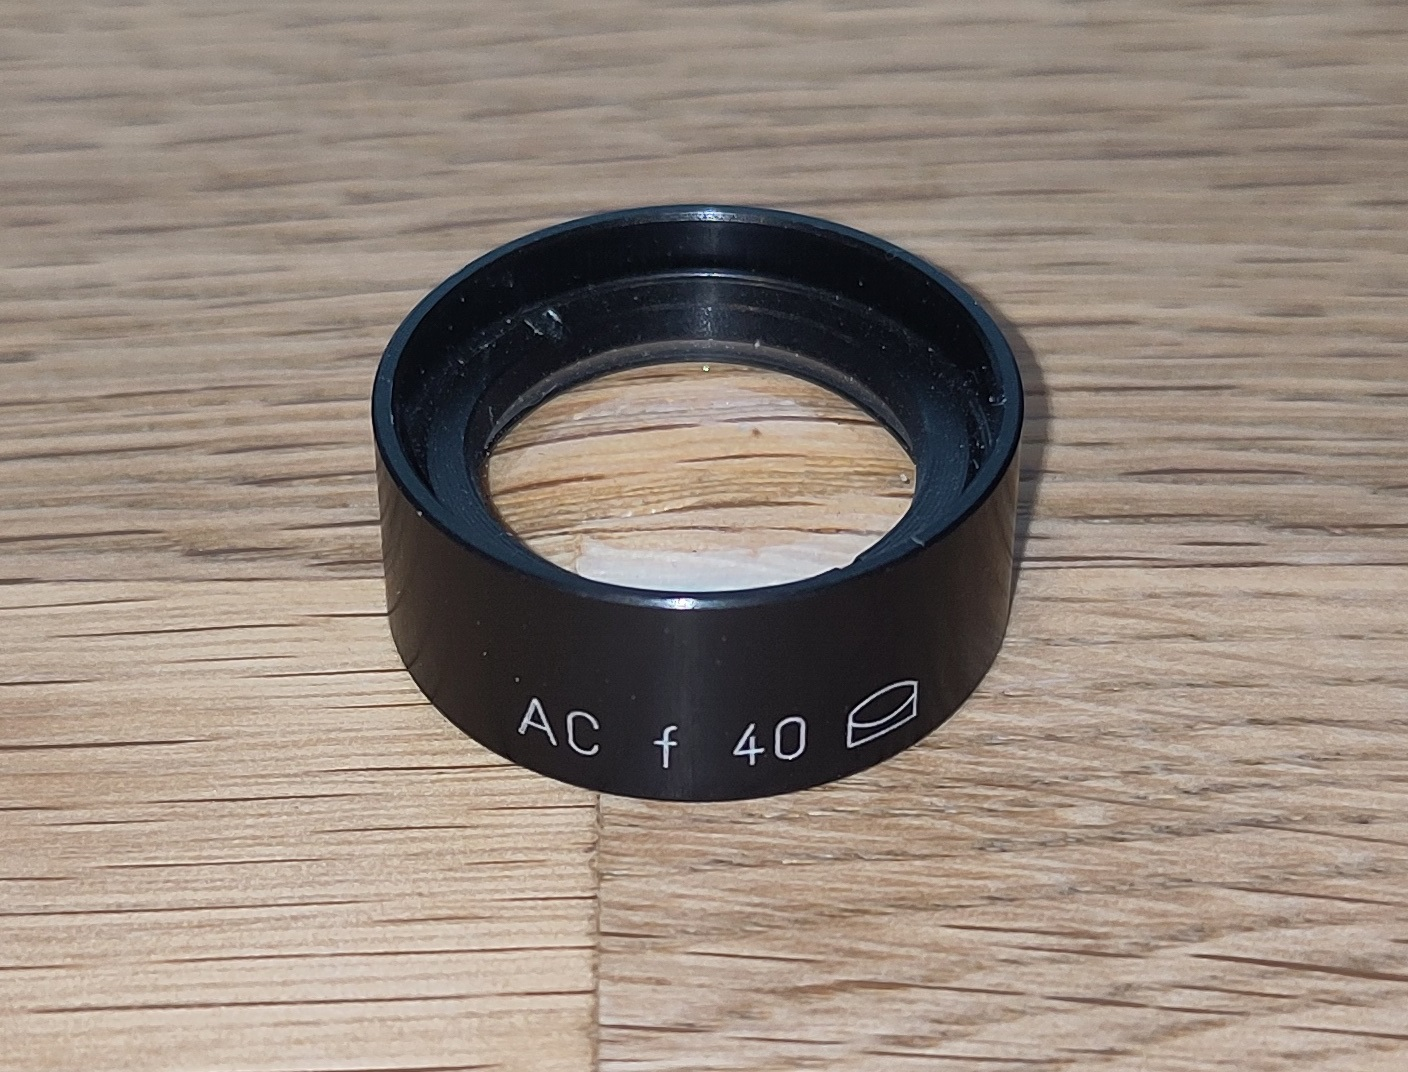
\includegraphics[width=0.5\textwidth]{../graphics/photo_lens.jpg}
    \caption{Lens from QIOPTIQ}\label{fig:lens}
\end{figure}

This lens enlarges the effective area on which the photocurrent can be received. This results in
higher reception power, i.e. a higher photocurrent.
The formula~\ref{eq:njl6401r3_lens} shows the increase in area to be expected when using such an optical system.

\begin{equation}\label{eq:njl6401r3_lens}
    A' = \frac{A_{L}}{A_{PD}} = \frac{(\frac{17~mm}{2})^2 \cdot \pi}{0.49~mm^2} = 463.2
\end{equation}
\myequations{Magnification of the receiving area by lens}

\subsubsection{Expected photocurrent}

Two scenarios are considered below: In the first, it is assumed, as before, that the light from the laser
propagates in a focused beam and then reflects off the target in a hemispherical and diffuse manner.

In the second scenario, an attempt is made to model the radiation pattern of the laser diode. According to the data sheet, the
diode has two different beam angles in the beam plane, which can be approximated with the solid angle of a rectangular pyramid.
Scattering is prevented because the beam is reflected by a mirror.

In both scenarios, the radiated power of the laser diode is higher than in the first calculation. In pulsed
operation, this can easily be increased above the maximum rating. Thermally, this does not pose a problem for the diode because
the duty cycle is very small. The formula~\ref{eq:rld65nzx1_higher_output} shows the new expected radiant power
of such a pulse. The efficiency of the laser diode is taken from the RLD65NZX1 data sheet \cite{rohm2019rld65nzx1_datasheet}.

\begin{equation}\label{eq:rld65nzx1_higher_output}
    \begin{split}
        \eta     & = \frac{P_{25~mA}}{I_{ld}} = \frac{7~mW}{25~mA} = 0.28~\frac{W}{A}   \\
        I_{ld}'  & = \frac{5~V - V_{LD}}{R_{v}} = \frac{5~V - 2.8~V}{5~\Omega} = 440~mA \\
        P_{out}' & = \eta \cdot I_{ld}' = 0.28~\frac{W}{A} \cdot 440~mA = 123~mW
    \end{split}
\end{equation}
\myequations{Increased transmission power of the laser diode}

For a target located at a distance of 2 meters, the following
photocurrent can be expected according to formula~\ref{eq:photocurrent_scenario1}:

\begin{equation}\label{eq:photocurrent_scenario1}
    \begin{split}
        P_{in} & = \frac{P_{out}}{\Omega \cdot r^2} \cdot A_{L} = \frac{123~mW}{4\pi \cdot 0.5~sr \cdot (2~m)^2} \cdot 227~mm^2 = 1.11~\mu W \\
        I_{ph} & = S \cdot P_{in} = 0.42~\frac{A}{W} \cdot 1.11~\mu W = 467~nA
    \end{split}
\end{equation}
\myequations{Photocurrent scenario 1}

Without optics, the laser diode does not emit a collimated beam. In the second scenario, this radiation pattern is modeled using
the solid angle of a pyramid, as defined in formula~\ref{eq:solid_angle_pyramid}. The typical
radiation angles $\theta$ are also taken from the laser diode data sheet. It should be noted that the
full angle is given in the data sheet. The value in the formula is therefore halved.

\begin{equation}\label{eq:solid_angle_pyramid}
    \Omega_{P} = 4 \cdot arcsin(sin(\theta_x) \cdot sin(\theta_y)) =  4 \cdot arcsin \parenth*{sin \parenth*{\frac{9\degree}{2}} \cdot sin \parenth*{\frac{29\degree}{2}}} = 4.2~sr
\end{equation}
\myequations{Laser diode radiation model}

The formula~\ref{eq:photocurrent_scenario2} is used again to calculate the expected received power and the corresponding
photocurrent. However, the difference to the previous calculation is that the solid angle must also be
taken into account before reflection. Therefore, the distance to the target is multiplied by two.

\begin{equation}\label{eq:photocurrent_scenario2}
    \begin{split}
        P_{in} & = \frac{P_{out}}{\Omega \cdot (2 \cdot r)^2} \cdot A_{L} = \frac{123~mW}{4.2~sr \cdot (2 \cdot 2~m)^2} \cdot 227~mm^2 = 416~nW \\
        I_{ph} & = S \cdot P_{in} = 0.42~\frac{A}{W} \cdot 416~nW = 175~nA
    \end{split}
\end{equation}
\myequations{Photocurrent scenario 2}

\pagebreak

\subsection{Transimpedance amplifier}

As the calculations in the previous chapters show, the photocurrents to be detected have very small
amplitudes. Furthermore, the light pulses are typically only of very short duration, namely in the range of a few nanoseconds.
As a result, the signals have correspondingly short rise times, which need to be detected.

The requirements indicate that an amplifier with a very high gain and a very high bandwidth must be used.
The amplifier circuit used is a current-to-voltage converter. Such a circuit of the operational amplifier,
as shown in Figure~\ref{fig:theory_tia}, is also called a transimpedance amplifier (\acrshort{tia}).

\begin{figure}[H]
    \centering
    \includegraphics[width=0.5\textwidth]{../diagrams/tia.pdf}
    \caption{Operational amplifier circuit as a \acrshort{tia}}\label{fig:theory_tia}
\end{figure}

As the name suggests, the transimpedance converter converts the photocurrent \lstinline|Id| into a voltage \lstinline|Vout|.
The feedback resistor \lstinline|Rf| determines the amplification factor, as the formula~\ref{eq:tia_simple}
shows:

\begin{equation}\label{eq:tia_simple}
    V_{out} = -R_{f} \cdot I_{d}
\end{equation}
\myequations{Übertragungsfunktion \acrshort{tia}}
